\documentclass{article}
\usepackage{amsmath}
\usepackage{caption}
\usepackage{graphicx}
\usepackage{pgfplotstable}
\usepackage{booktabs}
\usepackage{placeins}
\title{Document}
\author{Aditya Yadav}
\begin{document}
\maketitle
\section{Table}
\begin{table}[h!]
\centering
\caption{Heart Data}
\pgfplotstabletypeset[
col sep=space,
header=true,
string type,
]{heart.csv}
\end{table}
\section{Graphs}
\begin{figure}[h]
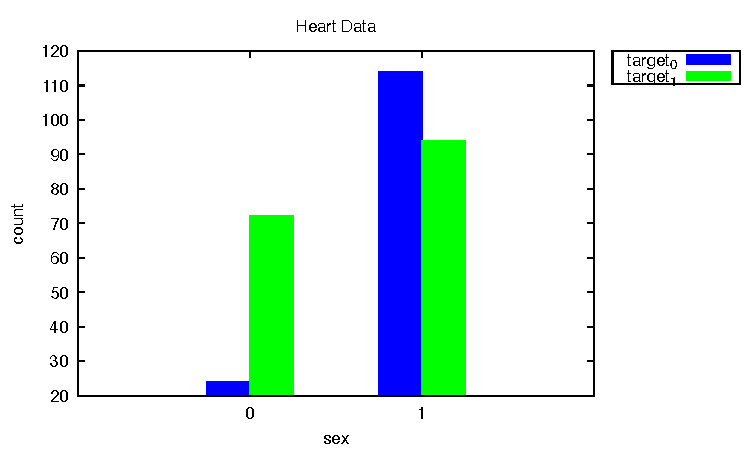
\includegraphics[width=\textwidth]{./.output_graph_q4_a.pdf}
\caption{\label{graph_1} Graph 1}
\end{figure}
\begin{figure}[h]
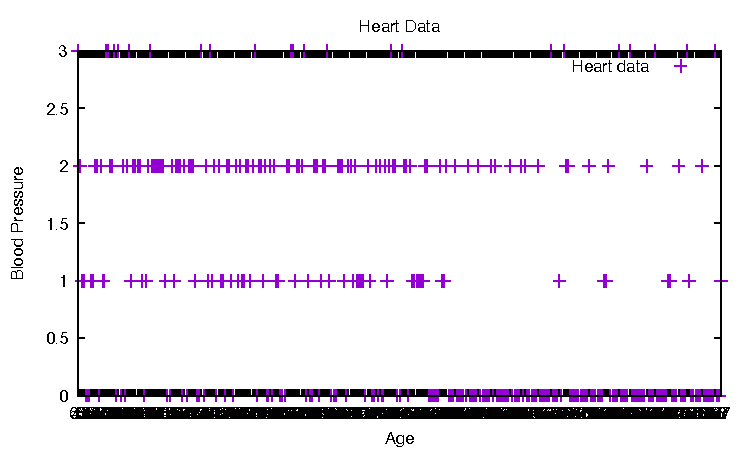
\includegraphics[width=\textwidth]{./.output_graph_q4_b.pdf}
\caption{\label{graph_2} Graph 2}
\end{figure}
\begin{figure}[h]
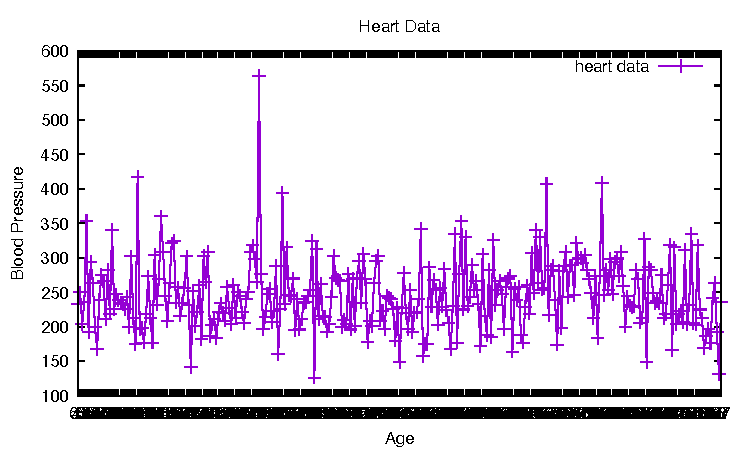
\includegraphics[width=\textwidth]{./.output_graph_q4_c.pdf}
\caption{\label{graph_3} Graph 3}
\end{figure}
\begin{figure}[h]
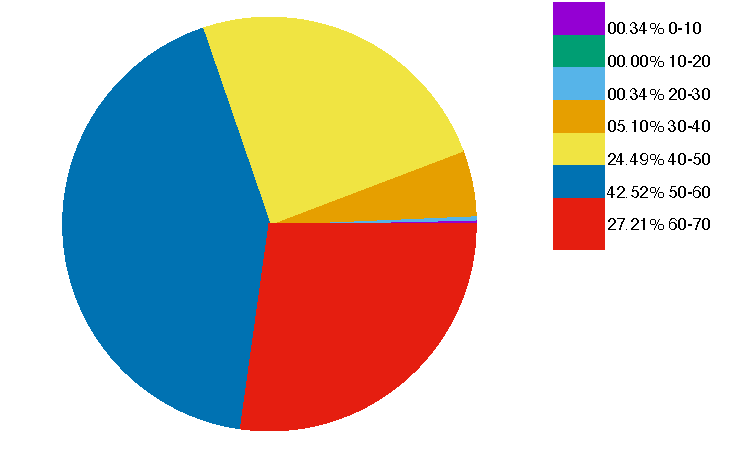
\includegraphics[width=\textwidth]{./.output_graph_q4_d.pdf}
\caption{\label{graph_4} Graph 4}
\end{figure}
\section{References}
Graph \ref{graph_1} shows histogram of gender vs number of people having heart disease. Graph \ref{graph_2} shows correlation between age and blood pressure. Graph \ref{graph_3} shows correlation between age and cholestrol. Graph \ref{graph_4} shows pie chart of age groups having heart disease.
\end{document}